 
\documentclass[12pt]{article}
%authors Andrew Schneider, David Dobor
\usepackage[margin=1in]{geometry} 
\usepackage{amsmath,amsthm,amssymb}
 \usepackage{graphicx}
 \usepackage{multirow}
\usepackage[scaled]{helvet}
\usepackage{hyperref}
\usepackage[usenames,dvipsnames,svgnames,table]{xcolor}
\usepackage[T1]{fontenc}
\usepackage{palatino}
\usepackage{enumerate}
%\renewcommand*\familydefault{\sfdefault} %% Only if the base font of the document is to be sans serif

\newcommand{\N}{\mathbb{N}}
\newcommand{\Z}{\mathbb{Z}}


\newcommand{\blditA}{\textbf{\textit{A}}}
\newcommand{\blditB}{\textbf{\textit{B}}}
\newcommand{\blditC}{\textbf{\textit{C}}}
\newcommand{\blditP}{\textbf{\textit{P}}}
\newcommand{\blditQ}{\textbf{\textit{Q}}}
\newcommand{\bldI}{\textbf{I}}
\newcommand{\blditX}{\textbf{\textit{X}}}
\newcommand{\blditY}{\textbf{\textit{Y}}}
\newcommand{\blditZ}{\textbf{\textit{Z}}}
 
\newenvironment{theorem}[2][Theorem]{\begin{trivlist}
\item[\hskip \labelsep {\bfseries #1}\hskip \labelsep {\bfseries #2.}]}{\end{trivlist}}
\newenvironment{lemma}[2][Lemma]{\begin{trivlist}
\item[\hskip \labelsep {\bfseries #1}\hskip \labelsep {\bfseries #2.}]}{\end{trivlist}}
\newenvironment{exercise}[2][Exercise]{\begin{trivlist}
\item[\hskip \labelsep {\bfseries #1}\hskip \labelsep {\bfseries #2.}]}{\end{trivlist}}
\newenvironment{problem}[2][Problem]{\begin{trivlist}
\item[\hskip \labelsep {\bfseries #1}\hskip \labelsep {\bfseries #2.}]}{\end{trivlist}}
\newenvironment{question}[2][Question]{\begin{trivlist}
\item[\hskip \labelsep {\bfseries #1}\hskip \labelsep {\bfseries #2.}]}{\end{trivlist}}
\newenvironment{answer}[2][Answer]{\begin{trivlist}
\item[\hskip \labelsep {\bfseries #1}\hskip \labelsep {\bfseries #2.}]}{\end{trivlist}}

\begin{document}
 \renewcommand{\arraystretch}{1.3}
 \renewcommand{\thefootnote}{\fnsymbol{footnote}}	
 
\title{Stat 8003, Homework 7}%replace X with the appropriate number
\author{Group G: \ \ \texttt{sample( c( "David" , "Andrew",  "Salam" ) )}
\\ %replace with your name
} %if necessary, replace with your course title
 
\maketitle
 
 %%%%%%%% Question 1 %%%%%%%%%
 \begin{question}{7.1} We want to know the mean percentage of butterfat in milk produced by a farm by sampling
multiple loads of milk. Previous records indicate the average percent butterfat in milk is 3.35
and the standard deviation among loads is 0.15. Now we hope to detect a change of the percent
butterfat in milk.  

\begin{enumerate}[(a)]
\item Find the rejection region at the significance level $\alpha = 0.05$;
\item Suppose 100 loads of milk are sampled. What is the power for the test for detecting a change of the mean to 3.40.
\item Plot the power as a function of the absolute value of the change in the mean over the standard deviation (which is $ | \mu_1 - \mu_0 | / \sigma$).
\item Now we hope to detect a change of the percent butterfat in milk to 3.40 with a power 0.8. How many loads do we need to sample?
\end{enumerate}

\end{question} 


  \textbf{\color{TealBlue}\emph{Answer:} } 
 \begin{enumerate}[(a)]  
%%%%%%%%%%%% answer to 1a %%%%%%%%%%%%
\item Let \texttt{r.v.} $X$ be the percentage of butterfat in milk.  We have
$$
X \sim N(\mu = 3.35, \sigma = 0.15)
$$
Or
$$
Z = \frac{X - 3.35}{0.15} \sim N(0,1)
$$
The null hypothesis is that there is no change in butterfat; the alternative hypothesis is that there is:
\begin{align*}
H_0 : \; \mu &= 3.35 \\
H_a : \; \mu &\neq 3.35\\
\end{align*}
The rejection region of this two sided test is given by 
\begin{align*}
\mathcal{R}  &= \Big\{ |\ Z \ | > z_{\alpha / 2} \Big\}  \\
&= \Big\{ Z < z_{0.975} \Big\} \cup \Big\{ Z >  z_{0.025} \Big\} \\
&= \Big\{  \frac{X - 3.35}{0.15} < - z_{0.025} \Big\}   \cup \Big\{  \frac{X - 3.35}{0.15} >  z_{0.025} \Big\} \\
&= \Big\{  \ X < 3.35 - 0.15 \times 1.96 \Big\}  \cup \Big\{ \ X >  3.35 + 0.15 \times 1.96 \Big\} \\
&= \Big\{  \ X < 3.056  \Big\}  \cup \Big\{ \ X > 3.644 \Big\} \\
\end{align*}

%%%%%%%%%%%% answer to 1b %%%%%%%%%%%%
\item We want the probability of rejecting the null when $H_a$ is true (specifically, when $\mu = 3.40$). With 100 loads of milk sampled, $\bar X \sim N(\mu, \sigma / \sqrt{ 100})$.
%\footnote{
%The rejection region for the mean of the 100 samples under $H_0$ is:
%
%\begin{align*}
%\mathcal{R} &= \Big\{  \frac{\bar X - 3.35}{0.015} < - z_{0.025} \Big\}   \cup \Big\{  \frac{\bar X - 3.35}{0.015} >  z_{0.025} \Big\} \\
%&= \Big\{  \ \bar X < 3.35 - 0.015 \times 1.96 \Big\}  \cup \Big\{ \ \bar X >  3.35 + 0.015 \times 1.96 \Big\} \\
%&= \Big\{  \ \bar X < 3.3206  \Big\}  \cup \Big\{ \ \bar X > 3.3794 \Big\} \\
%\end{align*}
%}

The probability of rejecting $H_0$ when in fact $\mu = 3.40$:
\begin{align*}
1 - \beta &= P\ \left( \ \mathcal{R} \mid \mu = 3.4 \ \right) = P \left( \ \Big| \frac{\bar X - 3.35}{0.015} \Big| > z_{0.025} \ \right)\\
&= P \ \left( \ \Big| \frac{\bar X - 3.4 + (3.4 - 3.35)}{0.015} \Big| > 1.96 \ \right) \\
&= P \ \left( \ \Big| Z +\frac{(3.4 - 3.35)}{0.015} \Big| > 1.96 \ \right) \\
&= P \ \left( \ Z > 1.96 - \frac{(3.4 - 3.35)}{0.015} \right) + P \ \left( \ Z < -1.96 - \frac{(3.4 - 3.35)}{0.015} \ \right) \\
&= P \ \left( \ Z > -1.373333 \ \right) + \text{\texttt{(negligible quantity)}} \\
&= \text{\texttt{1 - pnorm(-1.373333)}}
\end{align*}
$$
\boxed{\text{power}  = 1 - \beta  = 0.915}
$$

\item We now we express the power in terms of the absolute change in the mean over its standard deviation ( $ | \mu_1 - \mu_0 | / \sigma$) and plot the result.
\begin{align*}
1 - \beta &= P \left( \ \Big| \frac{\bar X - \mu_1 + (\mu_1 - \mu_0)}{\sigma} \Big| > z_{0.025} \right) \\
&= P \left( \ \Big|  Z +  \frac{\mu_1 - \mu_0} {\sigma}  \Big| >  1.96 \right) \\
&= P \left( \ Z > 1.96 -  \frac{ | \mu_1 - \mu_0 | } {\sigma}  \ \right)  + P \left( \ Z < -1.96 -  \frac{ | \mu_1 - \mu_0 | } {\sigma}  \right)  \\
&= \text{\texttt{1 - pnorm(1.96 - xaxis)}} + \text{\texttt{pnorm(-1.96 - xaxis)}} \\
\end{align*}

\begin{center}
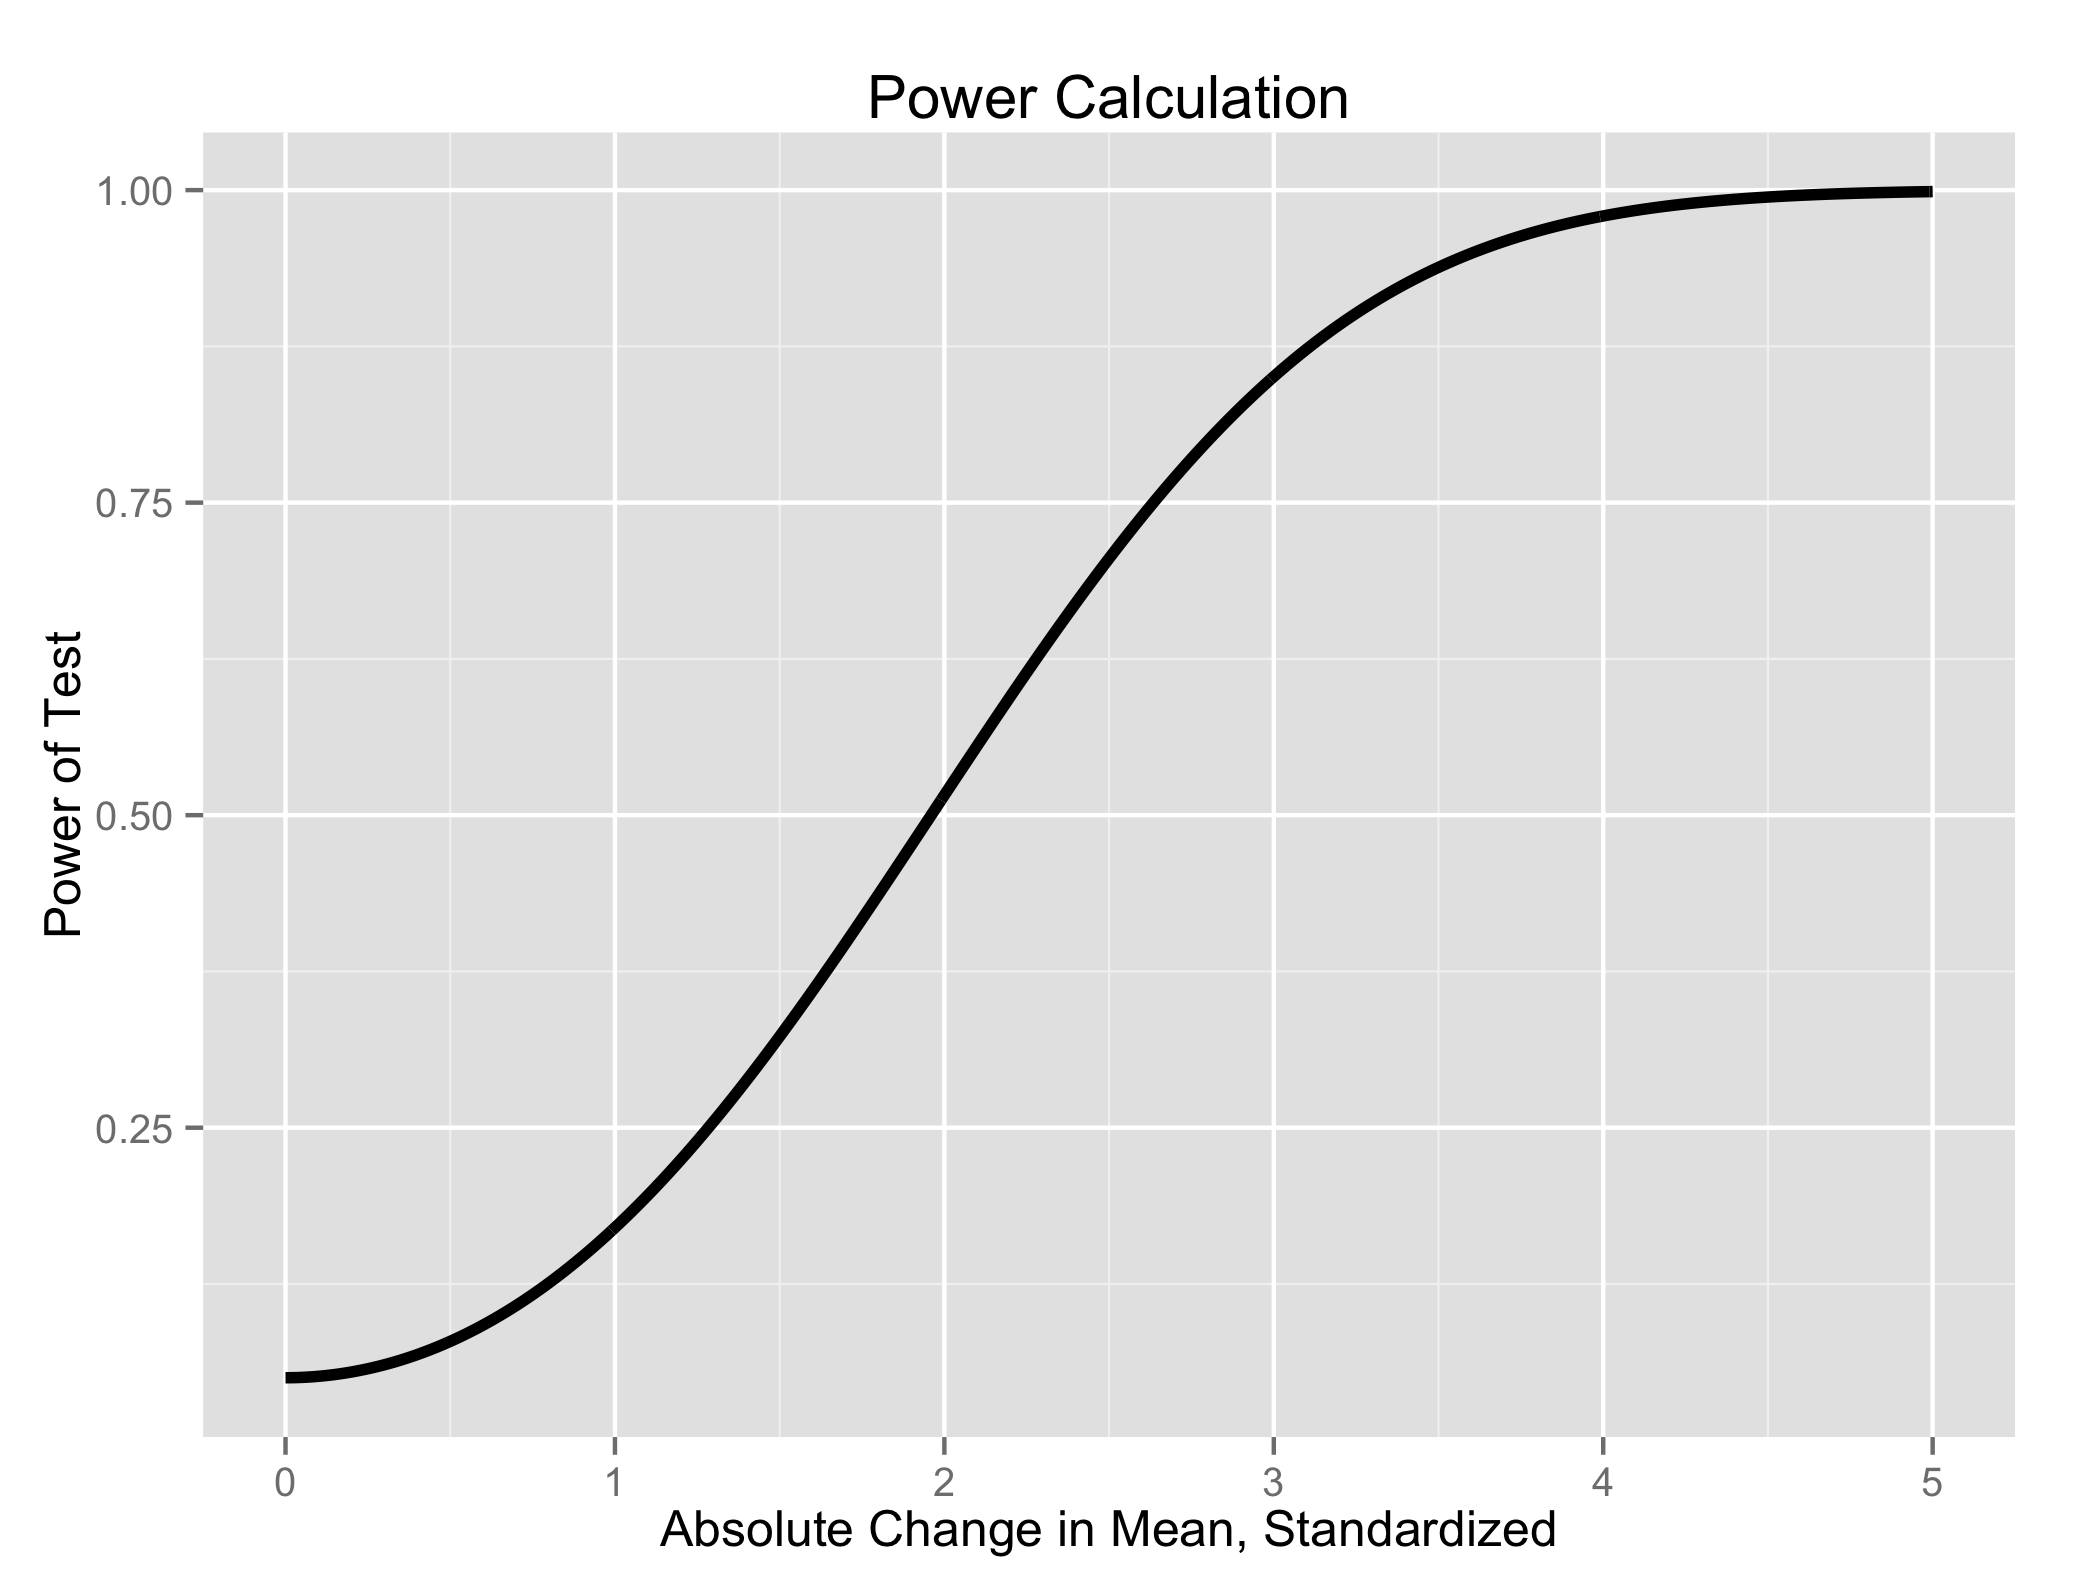
\includegraphics[width=10cm, height=8cm, width= 10cm]{power_plot_2c}
\end{center} 

\item Using the result obtained in class with $1 - \beta = 0.8$, we get:
\begin{align*}
n &= \frac{\sigma^2}{\delta^2} (z_{\frac{\alpha}{2}}+ z_{\beta})^2 \\
&= \frac{0.15^2}{(3.40 - 3.35)^2 }(z_{0.025} + z_{0.2})^2 \\
\end{align*}
$$
\boxed{n = 71}
$$

\end{enumerate}
\bigskip
\bigskip
 %%%%%%%% Question 2 %%%%%%%%%
 \begin{question}{7.2}  The relative rotation angle between the $\mathbf{L2}$ and $\mathbf{L3}$  lumbar vertebrate is defined as the acute
angle between posterior tangents drawn to each vertebra on a spinal $\mathbf{X}$-ray. When this angle is too
large the patient experiences discomfort or pain. Chiropractic treatment of this condition involves
decreasing this angle by applying (nonsurgical) manipulation or pressure. Harrison et al. (2002)
propose one such particular treatment. They measured the angle on both pre- and post-treatment
$\mathbf{X}$-rays from a random sample of 48 patients. At $\alpha = 0.05$, test whether the mean post-treatment
angle is less than the mean angle prior to treatment.

%
%You can load the data using the following command:
%
%
%\texttt{har <- read.table("http://astro.temple.edu/~zhaozhg/Stat8003/data/har1.csv", sep=",", header=TRUE)}
\end{question} 

  \textbf{\color{TealBlue}\emph{Answer:} } 

\bigskip
%%answer to 2 
We are comparing the means of pre- and post-treatment angles. 
Let the null hypothesis be that there is no change in the mean angle between pre- and post-treatments. We are testing for the left-sided alternative that there's  a decrease in the angle.  
\begin{align*}
H_0 : \; \; \mu_{\text{post}} = \mu_{\text{pre}}  \\
H_a:  \; \; \mu_{\text{post}} < \mu_{\text{pre}}  \\
\end{align*}
We first check whether the variances of the two groups are equal ($\sigma_{\text{post}} = \sigma_{\text{pre}} $) using the $F$-test. 

The $F$-statistic with 47 and 47 degrees of freedom returned by the $F$-test is 1.3369 and the $p$-value is 0.1615073. This $p$-value is too high offering us little evidence that the variances are different.  We thus \emph{accept} the hypothesis that the variances of the two groups are equal.

%We next proceed with the $T$-test. Using the notation $\bar y_{\text{pre}}$ and $\bar y_{\text{post}}$ for the sample means of the two groups  and $s_p$ for the pooled variance, we compute the following $T$-statistic with 47+47-2 degrees of freedom:
%\begin{align*}
%T = \frac{\bar y_{\text{pre}} - \bar y_{\text{post}} }{s_p\  /\  \sqrt{\frac{1}{48} + \frac{1}{48}}}
%\end{align*}

We use \texttt{R}'s paired T-test to see whether the mean post-treatment
angle is less than the pre-treatment mean angle:
\begin{verbatim}
t.test( har$Post, har$Pre, var.equal=TRUE, 
             alternative="less", paired=TRUE)
\end{verbatim}

This outputs \texttt{ p-value = 0.0004353} and we therefore \emph{reject} the null hypothesis that the means are equal.
\bigskip
$$
\boxed{ \text{ Accept} \ H_1: \text{The post-treatment mean is smaller } }
$$
 

\bigskip
\bigskip
 %%%%%%%% Question 3 %%%%%%%%%
 \begin{question}{7.3}This problem will guide you in demonstrating the multiplicity issues in multiple hypothesis testing using simulation. Let $X_{ij}$ be the data modeled as
\begin{equation}
X_{ij} \stackrel{iid}{\sim} N( \theta_j, 1 ), \; \; i = 1, 2, \dots , n \; \; \; j = 1,2,\dots, p.
\end{equation}

Consider testing $p$ hypotheses $H_{0j} : \theta_j = 0 \; \; vs H_{1j} : \theta_j \neq 0$ where $j = 1, 2, \dots, p$. Define the family-wise error rate (FWER) as
$$
FWER = P\ ( \text{at least one (including one) false rejection} \ ).
$$
Set the sample size $n = 50\ $ and $\alpha = 0.05$.
\begin{enumerate}[(a)]
\item Set $p = 1, \ \theta_j = 0,\  \forall j$. Generate $X_{ij}$ according to (1) and use $p$-value to test the hypothesis at $\alpha$-level. Replicate this step 1000 times to get the simulated FWER.
\item  Set $p = 10, \ \theta_j = 0,\  \forall j$. Generate $X_{ij}$ according to (1) and use $p$-value to test 10 hypothesis at $\alpha$-level. Replicate this step 1000 times to get the simulated FWER.
\item  Set $p = 100, \ \theta_j = 0, \ \forall j$. Generate $X_{ij}$ according to (1) and use $p$-value to test 100 hypothesis at $\alpha$-level. Replicate this step 1000 times to get the simulated FWER.
\item  Set $p = 100, \ \theta_j = 0, \ \forall j$. Generate $X_{ij}$ according to (1) and use $p$-value to test 100 hypothesis using Bonferroni's correction by setting the significance level at $\alpha / p$ for each hypothesis.  Replicate this step 1000 times to get the simulated FWER.

\end{enumerate}

\end{question} 
  \textbf{\color{TealBlue}\emph{Answer:} } 
  \bigskip
  
   To answer this question,  we wrote an \texttt{R} function that we use for parts (a) through (d). This function tests any number of hypotheses on a batch of 50 random numbers drawn from the standard normal distribution, where each hypothesis being tested is whether the mean of these 50 numbers equals zero, at a specified level of significance $\alpha$ (please see attached code for details). 
   
  Letting ${X_1, X_2, \dots, X_{n =50}}$ be a random sample from a $N(\theta, 1)$ population,
we reject $H_0 : \theta = 0$ in favor of $H_1 : \theta \neq 0$ whenever 
 $$
 | Z | = \Big| \frac{\bar X - \theta}{ 1 / \sqrt n} \Big| = \sqrt {50}\  | \bar X | \geq z_{0.025} = 1.96, 
 $$
 i.e. whenever
 $$
 \{ \bar X  \leq - 0.27719 \} \cup \{ \bar X \geq 0.27719 \} .
 $$


\begin{enumerate}[(a)]  
\item We first test a single hypothesis $H_0 : \theta = 0$ on one batch of 50 standard normals and \emph{accept} it. 

We then repeat this step 1000 times and get the result that about \fbox{0.044} of these hypotheses are rejected. (Of course this number varies with each run of the simulation, but it remains close to 0.05, as expected.)

\item We now test 10 hypotheses for each of the 1000 simulations. For each simulation run, we determine whether any of the 10 hypotheses have been rejected. Whenever at least one of the hypotheses is rejected, it contributes to the family wise error rate (FWER). 

At the end of this process, we find that \fbox{FWER = 0.39} - roughly a ten-fold increase from the result in part (a). (Again, this number varies slightly from one run to another).
\item We rerun part (b), this time with 100 hypotheses and find that the \fbox{FWER shoots up to 0.995}.
\item Finally, using the suggested Bonferroni's correction, we set $\alpha = 0.05/100$ and rerun part (c). We see that we are now \fbox{down to FWER = 0.033}.

\end{enumerate}
\end{document}

